\documentclass{standalone}
\usepackage{tikz}
\usepackage{tikz-qtree}
\usepackage[makeroom]{cancel}
\usetikzlibrary{fit}

% ОПИСАНИЕ: рекурсивный поиск схожести подвыражений
\begin{document} 
	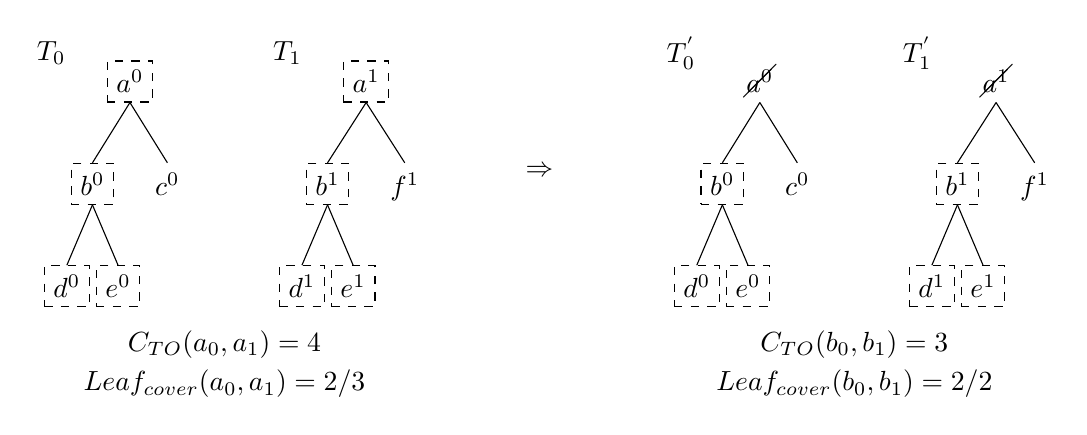
\begin{tikzpicture}[level distance=1.3cm]

		\node (cto1) at (1.2,-3.2) {$C_{TO}(a_0,a_1) = 4$};
		\node (lc1) at (1.2,-3.7) {$Leaf_{cover}(a_0,a_1) = 2/3$};

	    \node (x) at (-1,0.5) {$T_0$} ;
	    \Tree [.\node[draw,dashed]{$a^0$}; 
	            [.\node[draw,dashed]{$b^0$}; 
	                [.\node[draw,dashed]{$d^0$}; ] [.\node[draw,dashed]{$e^0$}; ] ] 
	            [.$c^0$ ]]]
	          
	    \begin{scope}[xshift=3cm]
	    \node (x) at (-1,0.5) {$T_1$} ;
	    \Tree [.\node[draw,dashed]{$a^1$}; 
	            [.\node[draw,dashed]{$b^1$}; 
	                [.\node[draw,dashed]{$d^1$}; ] [.\node[draw,dashed]{$e^1$}; ] ] 
	            [.$f^1$ ]]]
	    \node (x) at (2.2,-1) {$\Rightarrow$} ;
	    \end{scope}


	    \begin{scope}[xshift=8cm]

	    \node (cto2) at (1.2,-3.2) {$C_{TO}(b_0,b_1) = 3$};
		\node (lc2) at (1.2,-3.7) {$Leaf_{cover}(b_0,b_1) = 2/2$};

	    \node (x) at (-1,0.5) {$T_0^{'}$} ;
	    \Tree [.\cancel{$a^0$}
	        [.\node[draw,dashed]{$b^0$}; 
	            [.\node[draw,dashed]{$d^0$}; ] [.\node[draw,dashed]{$e^0$}; ] ] 
	        [.$c^0$ ]]]
	    \end{scope}

	    \begin{scope}[xshift=11cm]
	    \node (x) at (-1,0.5) {$T_1^{'}$} ;
	    \Tree [.\cancel{$a^1$}
	            [.\node[draw,dashed]{$b^1$}; 
	                [.\node[draw,dashed]{$d^1$}; ] [.\node[draw,dashed]{$e^1$}; ] ] 
	            [.$f^1$ ]]]
	    \end{scope}
	\end{tikzpicture}
\end{document} 